\documentclass[journal]{IEEEtran}
\usepackage{blindtext}
\usepackage{graphicx}


\ifCLASSINFOpdf
\else
\fi

\begin{document}
\title{ LinkedIN Career Path Recommendation\\
\begin{large} 
  \textbf{Algorithm on Big Data Optimization}
\end{large}
\\
\begin{large} 
  \textbf{School of engineering and applied sciences}
\end{large} 
}


\author{Deval~Shah,{1401060}}% <-this % stops a space


\markboth{Final Examination | April 28 , 2017}%
{Shell \MakeLowercase{\textit{et al.}}: Bare Demo of IEEEtran.cls for Journals}




\maketitle


\begin{abstract}
In this report , problem of modelling career paths for user's based on their prior information of their profiles is addressed.Data is available of different professions in computer industry.Data is passed through reduction,cleaning and filtering modules for preprocessing.After filtered data is available in proper format we apply clustering algorithm for avoiding mismatch of user's current position in industry with database.Ground Truth Data is constructed to check what minimum influential factors user require to progress in career path.Graph search technique is used to do factor matching between positions in job.As a conclusion, we will analyze the results and discuss possible improvements of our model. 
\end{abstract}

\begin{IEEEkeywords}
Clustering,Ground Truth Construction,Influential factors,Graph-Hash search
\end{IEEEkeywords}


\section{\textbf{Introduction}}
\subsection{\textbf{Problem Definition}}
LinkedIN company has million of user's using the platform daily.Many job hunters visit the site everyday for finding new jobs catering the skills they already have.If a user already is employed what can site do to help a user progress in career?.There are two ways in which this problem can be addressed 
\\
\\1. Reading user's profile and recommending a set of skills
\\2. User giving input as career goal and output should be career path for it.


\section{\textbf{Data}}  
    \subsection{\textbf{Data Collection}}
    \\The candidate profile data is provided having 38 text files with each file representing a profession in computer industry.Each file has a list of candidates having different jobs in that particular profession.
    \subsection{\textbf{Data Preprocessing}}
    After collection of data ,it is preprocessed for transforming it to structure the data,reducing it to work with only relevant attributes in data and cleaning to process data in python.
    \subsubsection{\textbf{Data Transformation}}
        All 38 text files of data of size 4.08 MB are merged together and converted into single json file (3.97 MB).    
    \subsubsection{\textbf{Data Reduction}}
        Attributes that are relevant to context of problem like skills,qualification,current job status etc. are kept and all other attributes are discarded.There is lot of information in user profile all of which is not relevant to skill recommendation like project description , duration of project , tools used in project etc.After data reduction file size is around ~662 KB which is almost 1/6 th of original data.         
    \subsubsection{\textbf{Data Cleaning}}
        Reduced Json file is passed into cleaning module where all noisy unicode strings present in files is converted to utf-8 encoding scheme for processing the data in python.After reduced data is cleaned it is stored in file system for processing.
    
    \begin{center}
        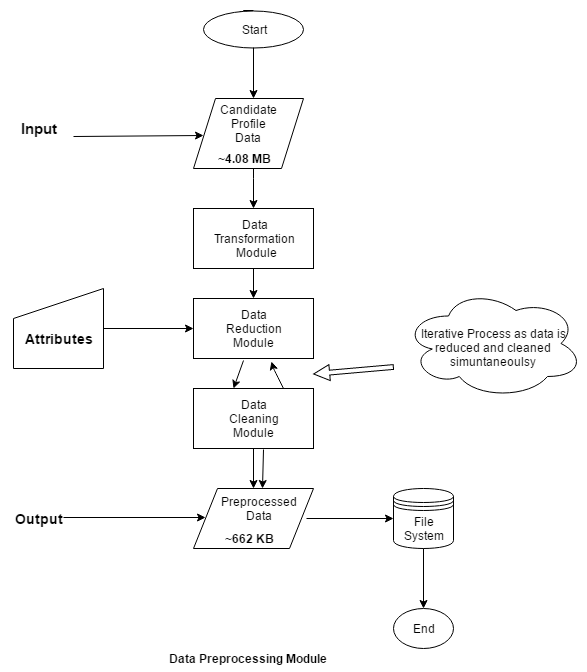
\includegraphics[scale=0.45]{Data_Preprocessing.png}
         \\\caption\textit{{Fig 1.Data Prepocessing module}}
    \end{center}
    
    \begin{center}
        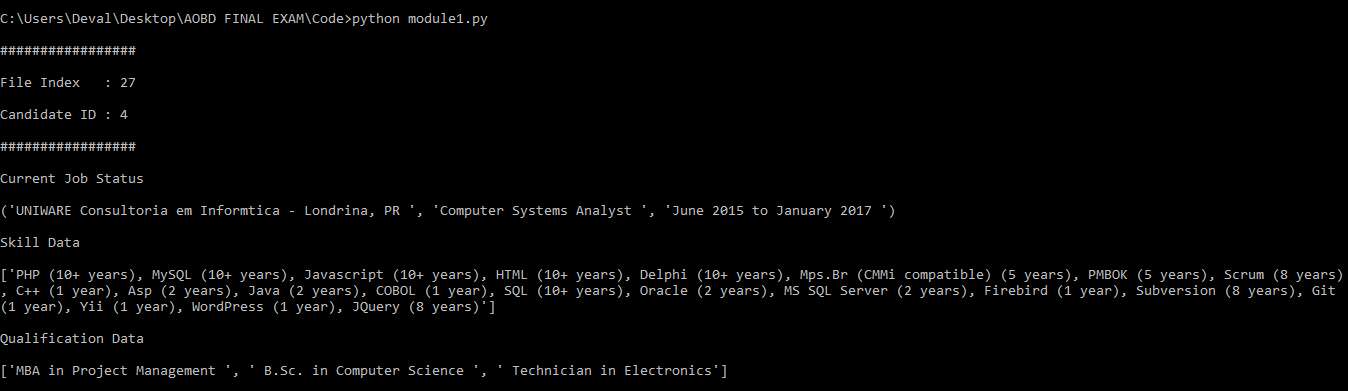
\includegraphics[scale=0.25]{index_2_cid_4.PNG}
        \\\caption\textit{{Fig 2.Output of data prepocessing module\\ Choosing a file index = 2 and candidate id = 4}}
    \end{center}
        
    \\\textbf{Challenges In Preprocessing Data}  
    The data from LinkedIN is represented in natural language format, and this added to the task of data cleaning an additional level of processing requirement. The entries in the raw data highly vary from person to person,depending on their input. Many job titles contain more details that are not specific or necessary(which is more general), e.g.
    computer engineer.Details like this make difficult for system to identify specific job position of user to recommend skills for the same.
    
\section{Techniques}
    
    Below are the techniques used to solve some issues encountered during  data preprocessing task and to use in matching algorithms used in module 1 and module 2.
    \subsubsection{\textbf{Semantic Similarity Matching}}
        After doing preprocessing on data,to avoid or improve natural language format used by users ,the idea is to do natural language processing on preprocessed data on attributes so that we can find all similar words using semantic similarity technique  
    
    \subsubsection{\textbf{Clustering}}
       Similar words obtained through semantic similarity matching technique is stored in cluster where the center would be word with highest similarity.These clustering is done by k-means clustering algorithm.
       After clustering, many semantically similar job titles are grouped together. For example, “software development engineer”, “programmer”, “software developer” are all grouped together with “software engineer”, and “Recruiting Coordinator”, “Technical Recruiter” are grouped with “Recruiter”.
        \begin{center}
            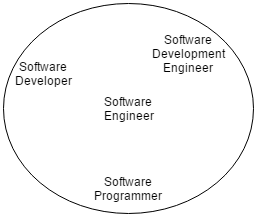
\includegraphics[scale=0.45]{clustering.png}
            \\\caption\textit{{Fig 3.Clustering semantically similar words}}
        \end{center}
   
   \subsubsection{\textbf{Influential Factors Identification}}
        To model a career path for user what prior knowledge you need to have is addressed in this technique.Attributes which influence the career path to go in certain orientation should be kept and others should be discarded.This technique is used in data preprocessing step where it has been identified through research that skills , qualification data ,current job status , location etc have proven to be most influential factors in identifying subsequent career choice.
        \begin{center}
        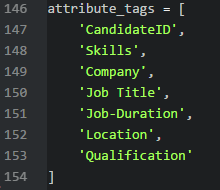
\includegraphics[scale=0.7]{attributes}
        \\\caption{\textit{Fig 4. Attributes selected for career path recommendation}}
        \end{center}
        
        
    \subsubsection{\textbf{Ground Truth Data Construction}}
        Ground truth refer to information provided by direct observation as opposed to information provided by inference.This technique is of the most important technique in terms of prior data construction that is needed for recommending career path.These data is not obtained from given data but is constructed to use for matching in algorithms to verify it.Based on prior knowledge, Roughly split each career path in our collected data into four stages, where each stage represents a milestone within the whole career path.For eg :- if we have a profession of software engineer than career path is given along with bare minimum skills required in each path,career level indicates what is the level of user currently and how much progress can it make before reaching top.Due to vocabulary variations,different users utilize different job titles to
        refer to the same career stage.For eg - programmer,developer etc.
        So we include all semantically similar words in career stages to avoid any conflict while matching. 
        
        \begin{center}
        \includegraphics[scale=0.345]{ground_truth}
        \caption{\textit{Fig 5.Ground Truth}}
        \end{center}
   
   \subsubsection{\textbf{Graph-Hash Search}}
        Let x0 node denote user's current career position.Now for each profession we create a separate graph where first node(root) would be level 0 career stage.Child of root node would be level 1 career stage and so on.Suppose there are m professions we get m such graphs.Each graph having 1 root(L0) and 3 children (L1,L2,L3) .
        Store each graph in hash table for unique identification of each profession.Now we can use user's profile parameters such as current job status data to exactly map to index where career path graph is located in hash table and use \textbf{breadth first search} to find which level node(user's current career stage in ground truth) does it belong to.By using skill data we can determine the difference score for which skills the user lacks in order to progress to next career stage and return that difference of skills. 
    
\section{\textbf{Algorithms}}

    \subsection{\textbf{Module 1}}
    Module that reads user’s profile and suggest a career path – in terms of skillset to be acquired.
    \\\textbf{Assumption} :All Career paths has four stage depth.(Ideal Scenario)Ground Truth Data assumes this.Real world data may vary with depths different in different scenario.        
        \\
        \subsubsection{\textbf{Algorithm Flowchart}}
        \\
            \begin{center}
                \includegraphics[scale=0.43]{Module_1.png}
                \\
                \caption{\textit{Fig 6. Module 1}}
            \end{center}
        \\
    
    \subsection{Module 2}
     A module in which user enters a career goal and based on this career goal and other related information the platform suggest a career path. 
     \\\textbf{Assumption} : User will enter career goal in two parts = industry to work in  + profession in that industry.(selects both from a predefined list).
     \\For eg : Data Scientist , Computer Science
     \\The career path is formed as a graph in output in which nodes represent different stages required by user to attain the career path.
     \\
        \subsubsection{\textbf{Algorithm Flowchart}}
        \\
            \begin{center}
                \includegraphics[scale=0.412]{Module_2.png}
                \\
                \caption{\textit{Fig 7. Module 2}}
            \end{center}
        \\  
\section{\textbf{Conclusion}}
The algorithm formulated for modules 1 and 2 are based on techniques discussed before and they work under giving assumptions only.Major challenge in solving this problem appears in data preprocessing phase where the data provided has many attributes which is natural language format hence it is very difficult for system to interpret or contextualize from it.Methods are presented where in system can avoid these issues to certain extent.Ground Truth Data sole purpose is to compare with output given by system.It is not inferred but constructed on facts for system.Solutions presented in this report are based on standard big data mining techniques.Graph hash search is my idea of combining fast hash search - O(1) and bfs node search O(V + E).
Also as number of industries and professions are going to be finite always and there will not be a chance of increasing space exponentially in hash table.

\\
\\
\\
\\\begin{thebibliography}{9}

\bibitem{Modelling career path} 
Ye Liu† , Luming Zhang , Liqiang Nie , Yan Yan , David S. Rosenblum
\textit{Fortune Teller: Predicting Your Career Path}. 
School of Computing, National University of Singapore, Singapore 2016
 
\bibitem{asas} 
Giannis Varelas , Epimenidis Voutsakis , Paraskevi Raftopoulou  
\\\textit{Semantic Similarity Methods in WordNet and their
Application to Information Retrieval on the Web}. 
Dept. of Electronic and Comp. Engineering, Technical University of Crete (TUC),  2005.
 
\bibitem{knuthwebsite} 
K-means clustering algorithm
\\\texttt{https://sites.google.com/site/dataclusteringalgorithms/k-means-clustering-algorithm}

\bibitem{knuthwebsite} 
Data Mining Book
\\\texttt{http://guidetodatamining.com/}
\end{thebibliography}

\end{document}


